% !TeX root = ./Dyplom.tex
% chktex-file 26

\chapter{Reprezentacja wektorowa}
	W zagadnieniach NLP (ang. \emph{Natural Language Processing}) słowa wyrażone są w postaci wektorów liczb rzeczywistych (ang.\ \emph{word embedding}).
	W powstałej przestrzeni odległość między wektorami reprezentującymi podobne słowa jest mniejsza, niż odległość między słowami o różnym znaczeniu.
	Tradycyjne metody opierają się na semantyce dystrybucyjnej.
	Zgodnie z tą teorią, słowa występujące w podobnym kontekście mają podobne znaczenie.
	Bazując na tej zasadzie skonstruowano wiele algorytmów, zdolnych do wygenerowania wektorów słów analizując dużą ilość nieustrukturyzowanych tekstów.
	Architektura takich modeli opiera się na sieciach neuronowych próbujących przewidzieć słowo w zależności od kontekstu
		(modele CBOW --- ang. \emph{Continuous bag-of-words}) lub kontekst w zależności od słowa (ang.\ \emph{skip-gram})\cite{word2vec}, gdzie kontekst to otaczające słowa.
	Wadą tych modeli jest fakt, że są one niekontekstowe.
	\todo{odnieść się do\cite{BoW_PL}}
	Oznacza to, że po nauczeniu modelu, gdy chcemy go wykorzystać do obliczenia wektora danego słowa, to otrzymany wektor nie bierze pod uwagę kontekstu, w jakim występuje to słowo.
	Przykładowo słowo ,,zamek'' będzie reprezentowane przez taki sam wektor niezależnie od tego,
		czy w danym zdaniu odnosi się do zabezpieczenia antywłamaniowego, czy też widowiskowej dolnośląskiej budowli obronnej.
	
	W 2018 r ukazała się praca prezentująca BERT (ang.\ \emph{Bidirectional Encoder Representations from Transformers})\cite{BERT}.
	Był to pierwszy model kontekstowy.
	Oparty jest na transformerach\cite{Transformers} --- mechanizmach wykorzystujących bloki atencji.
	Mechanizmy te wykrywają zależności między słowami w zdaniu.
	Do warstwy atencji wszystkie słowa wprowadzane są równolegle, a na wyjściu dla każdego słowa otrzymujemy ważoną sumę wektorów wszystkich słów.
	Im większe powiązanie słowa ze słowem analizowanym, tym większa waga.
	Przykład zilustrowany na rysunku~\ref{fig:attention} przedstawia wagi poszczególnych słów w zdaniu ,,The animal didn't cross the street because it was too tired'' w kontekście słowa ,,it''.
	Zaimek ten może odnosić się zarówno do zwierzęcia z początku zdania (ang.\ \emph{The animal}), jak i ulicy (ang.\ \emph{the street}).
	Mechanizm przypisał największą wagę do zwierzęcia, co jest poprawnym działaniem w kontekście tego zdania.
	\begin{figure}[ht]
		\centering
		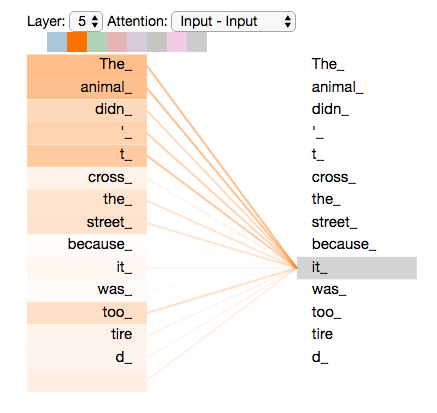
\includegraphics[width=.5\textwidth]{rys03/transformer_attention.png}
		\caption{Mechanizm atencji --- wizualizacja wag poszczególnych słów podczas analizy słowa ,,it''.
			Źródło: https://jalammar.github.io/illustrated-transformer}\label{fig:attention}
	\end{figure}
	
	Równoległe wprowadzanie wszystkich słów wymusza górne ograniczenie na długość zdania.
	Dla większości modeli bazujących na transformerach limit wynosi 512 tokenów.
	Tokenem może być zarówno słowo, jak i część zdania typu przecinek, stąd faktyczny limit liczony w słowach jest jeszcze niższy.
	Jest to mocno ograniczający limit w kontekście wykorzystywanego korpusu, w którym wypowiedzi często złożone są z kilkudziesięciu zdań.
	Problem ten opisywany jest szerzej w rozdziale~\ref{sec:sentences}.

\section{Wektory zdań}
	Modele bazujące na BERT stworzone są z myślą generowania wektorów dla każdego tokena wejściowego.
	Otrzymane w ten sposób wektory kodują informacje semantyczne o wszystkich słowach zdania, jednak nie zawierają informacji o samym zdaniu.
	Jedną z możliwości jest wykorzystanie wartości wektora dla tokena \verb|CLS| --- jest to token wykorzystywany podczas uczenia modelu i reprezentuje znaczenie zdania w kontekście zadań klasyfikacji.
	Można również uśrednić wektory wszystkich słów, jednak nie wszystkie słowa w zdaniu niosą tak samo dużo znaczenia.
	
	Rozwiązanie tego problemu proponują autorzy Sentence-BERT\cite{sbert}.
	Model SBERT złożony jest z dwóch modli BERT połączonych w syjamską sieć.
	Na wyjściu każdego modelu BERT dołożona jest warstwa pooling zwracająca wektor ustalonego rozmiaru dla zdań różnych długości.
	Najlepszą strategią okazała się metoda uśredniania wektorów wszystkich tokenów.
	Następnie wyjściowe dwa wektory wynikowe są łączone i obliczana jest funkcja straty klasyfikatorem \verb|softmax|.
	Architektura ta przedstawiona została na rysunku~\ref{fig:sbert}.
	W celu uzyskania wektorów kodujących semantykę całych zdań, model uczony jest na korpusach zawierających pary zdań oznaczone pod kątem podobieństwa.
	Optymalizuje się odległość między podobnymi zdaniami, jednocześnie maksymalizując odległości między zdaniami różnymi.
	\begin{figure}[ht]
		\centering
		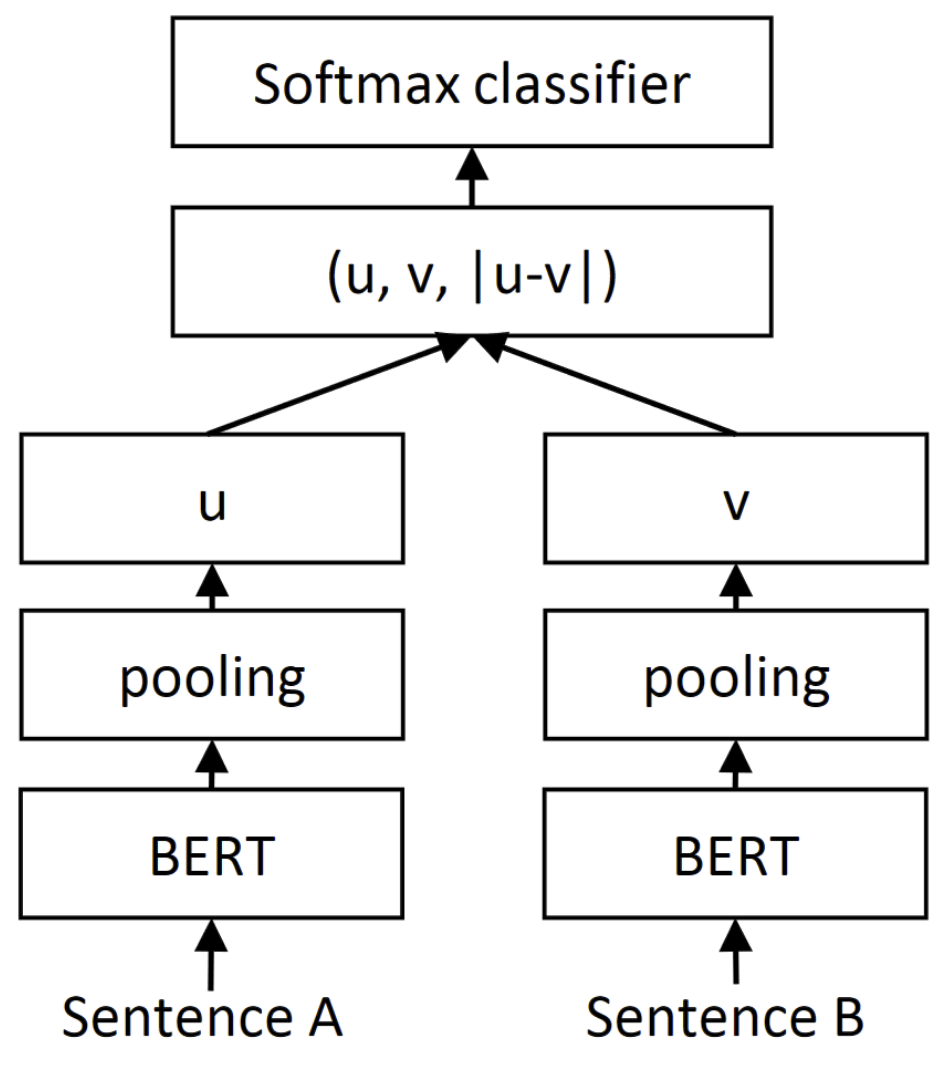
\includegraphics[width=0.3\linewidth]{rys03/sbert.png}
		\caption{Architektura modelu Sentence-BERT\cite{sbert}}\label{fig:sbert}
	\end{figure}

	Ze względu na specyfikę potrzebnego korpusu do trenowania modeli SBERT (oznaczone pary zdań) nie istnieją obecnie modele wytrenowane w języku polskim.
	Jednak w roku 2020 ci sami autorzy opracowali metodę przenoszenia wiedzy (ang.\ \emph{knowledge distillation}) z nauczonego modelu angielskiego na modele wielojęzykowe\cite{sbert_multilingual}.
	Opiera się na koncepcji, według której te same zdania w różnych językach powinny być reprezentowane przez podobne wektory w tej samej przestrzeni.
	Przekazanie wiedzy polega na minimalizacji różnicy wyników między modelem nauczającym, a modelem uczącym się (ang.\ \emph{teacher-student}) --- Rys.~\ref{fig:sbert_multilingual}.
	W tym przykładzie modelem-nauczycielem jest SBERT wytrenowany na angielskim korpusie, natomiast uczniem jest model XLM-R (XLM-RoBERTa).
	Jest to wielojęzykowy model bazujący na architekturze RoBERTa (wariacja BERT stworzona przez Facebook), wytrenowany na 2.5TB danych z CommonCrawl w 100 językach, w tym polskim\cite{xml_r}.
	Model ten zajmuje obecnie ósme miejsce w rankingu KLEJ\footnote{\url{https://klejbenchmark.com/leaderboard} (dostęp dnia 20 maja 2021)}
		oraz drugie miejsce po dostrojeniu (ang.\ \emph{fine-tuning}) na dodatkowych polskich korpusach.
	\begin{figure}[ht]
		\centering
		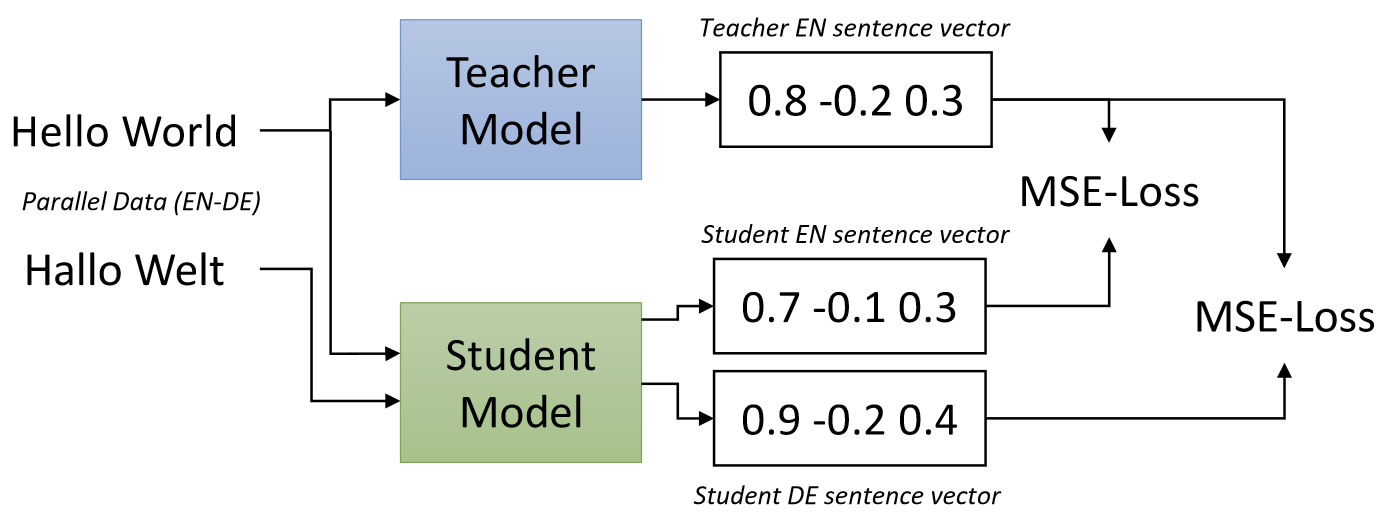
\includegraphics[width=.75\linewidth]{rys03/sbert_multilingual.png}
		\caption{Układ modeli nauczyciel-uczeń w procesie uczenia wielojęzykowego SBERT\cite{sbert_multilingual}}\label{fig:sbert_multilingual}
	\end{figure}
	
	Trenowanie modelu ucznia wymaga par zdań w języku angielskim i języku docelowym.
	Jest to dużo mniejsze ograniczenie, niż w przypadku bezpośredniego uczenia SBERT w docelowym języku.
	Dostępne są wytrenowane modele\footnote{\url{https://www.sbert.net/docs/pretrained_models} (dostęp dnia 20 maja 2021)}, które obejmują również język polski.
	Zostały one uwzględnione w rankingu modeli generujących reprezentacje zdań w języku polskim\cite{sentence_eval}.
	W pracy tej autorzy przetłumaczyli popularny angielski korpus SICK (ang.\ \emph{Sentences Involving Compositional Knowledge})
		zawierający pary zdań oznaczone pod kątem implikacji (ang.\ \emph{entailment}).
	Każda para może być albo powiązana (prawdziwość pierwszego zdania oznacza prawdziwość drugiego), neutralna (pierwsze zdanie nie mówi nic o prawdziwości drugiego), albo sprzeczna.
	Na podstawie tego korpusu stworzono dwa zadania odpowiadające angielskim --- SICK-E (zadanie klasyfikacji) oraz SICK-R (zadanie przewidywania dystrybucji podobieństwa, mierzone miarą korelacji Pearsona).
	
	Na potrzeby tej pracy za najbardziej istotne zadanie uznano SICK-R, ponieważ sprawdza skuteczność oceniania podobieństwa semantycznego dwóch tekstów.
	W tym zadaniu najlepszy wynik uzyskał wielojęzykowy model SBERT \verb|xlm-r-distilroberta-base-paraphrase-v1|
		(aktualne wyniki znajdują się na stronie z kodem źródłowym\footnote{\url{https://github.com/sdadas/polish-sentence-evaluation} (dostęp dnia 20 maja 2021)}).

\section{Wektory wypowiedzi}\label{sec:sentences}
	Modele bazujące na architekturze BERT mają górne ograniczenie na długość zdania wejściowego.
	Wynosi ono 512 tokenów, co odpowiada około 300 słowom.
	Dodatkowo, zbiór danych uczących wykorzystywanych przez modele SBERT zawiera zwykle krótsze zdania,
		przez co skuteczność tych modeli dla pełnego zakresu 512 tokenów może być gorsza niż oczekiwana.
	Jak pokazano na rysunku~\ref{fig:word_count}, wypowiedzi sejmowe są często znacznie dłuższe niż ten limit.
	Mediana liczby słów wynosząca 219 mieści się w limicie, jednak wypowiedzi złożone z więcej niż 300 słów stanowią prawie 39\% zbioru.
  \begin{figure}[ht]
    \begin{minipage}{.75\textwidth}
      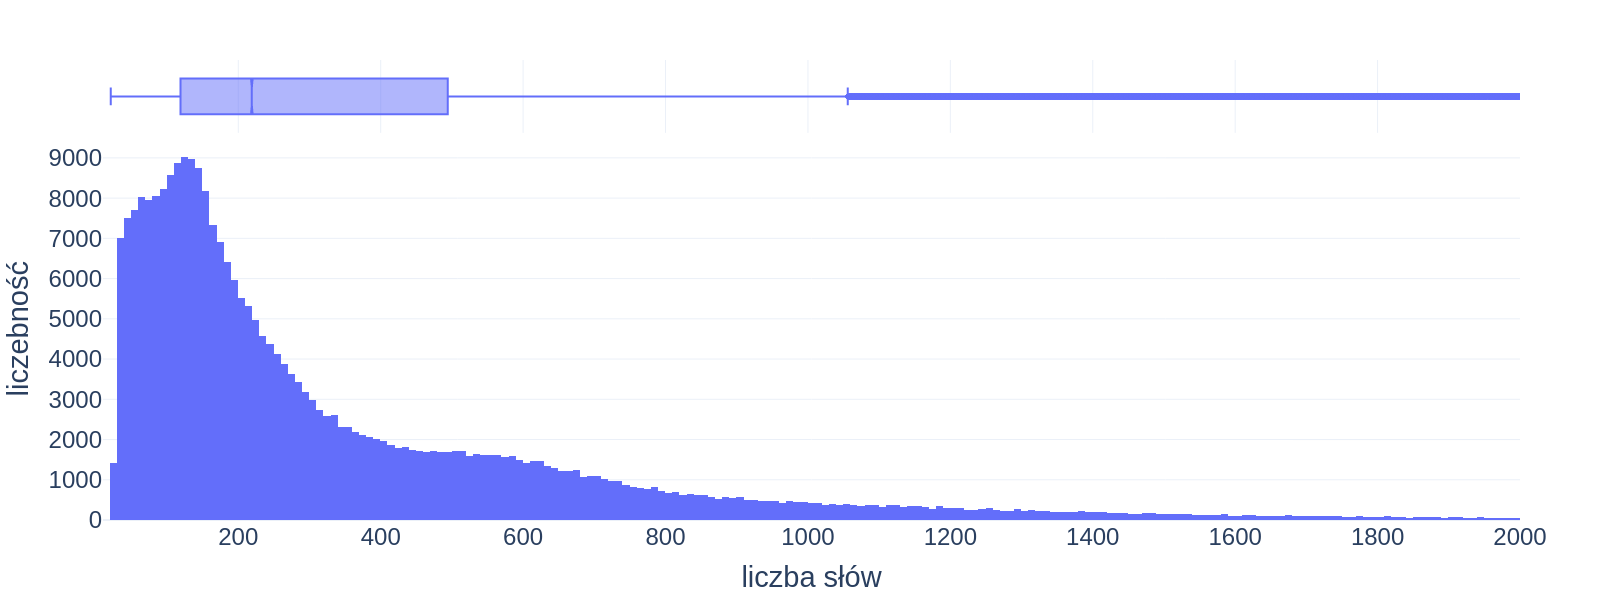
\includegraphics[width=\textwidth]{rys03/word_count.png}
    \end{minipage}%
    \begin{minipage}{.25\textwidth}
      \small
      \begin{tabularx}{\textwidth}{ll}
        Min & 21 \\ 
        Q1 & 119 \\ 
        Mediana & 219 \\
        Q3 & 494 \\ 
        Górny wąs & 1056 \\
        Max & 28.546 \\
      \end{tabularx}
    \end{minipage}
    \caption{Dystrybucja długości wypowiedzi (zakres do 2000 słów)}\label{fig:word_count}
  \end{figure}

	Z tego powodu postanowiono dzielić wypowiedzi na zdania, generować wektory dla każdego zdania, a następnie połączyć je w jeden wektor wynikowy dla całej wypowiedzi.
	Rozważono następujące strategie:
	\begin{itemize}
		\item średnia,
		\item średnia ważona,
		\item wektor pierwszy w rankingu,
		\item średnia pierwszych pięciu wektorów w rankingu
	\end{itemize}
	Do wygenerowania wag oraz rankingu potrzebna jest metoda oceniająca, na ile istotne jest każde zdanie w kontekście całej wypowiedzi.
	Stworzono w tym celu dwie metody: jedna wykorzystująca algorytm LexRank oraz druga wykorzystująca TF-IDF\@.

	\subsection{LexRank}
		LexRank\cite{LexRank} to stworzony w 2004r.\ stochastyczny algorytm bazujący na teorii grafów, służący do generowania podsumowań długich tekstów.
		Jako podsumowanie traktowany jest zbiór najistotniejszych zdań z tekstu --- jest to metoda ekstrakcyjna, która nie zmienia struktury zdań.
		Istnieją nowe metody bazujące na uczeniu maszynowym, które jako podsumowanie generują nowy tekst zawierający sens dokumentu,
			jednak na potrzeby tej pracy wymagany jest algorytm przypisujący wagi oryginalnym zdaniom.
		
		Algorytm konstruuje graf, gdzie wierzchołki odpowiadają zdaniom, a ich wartość obliczana jest algorytmem TF-IDF\@.
		Krawędzie grafu odpowiadają wartości podobieństwa między dokumentami i mierzone są na miarą kosinusową.
		Wizualizacja takiego grafu przedstawiona została na rysunku~\ref{fig:lexrank}.
		\begin{figure}[ht]
			\centering
			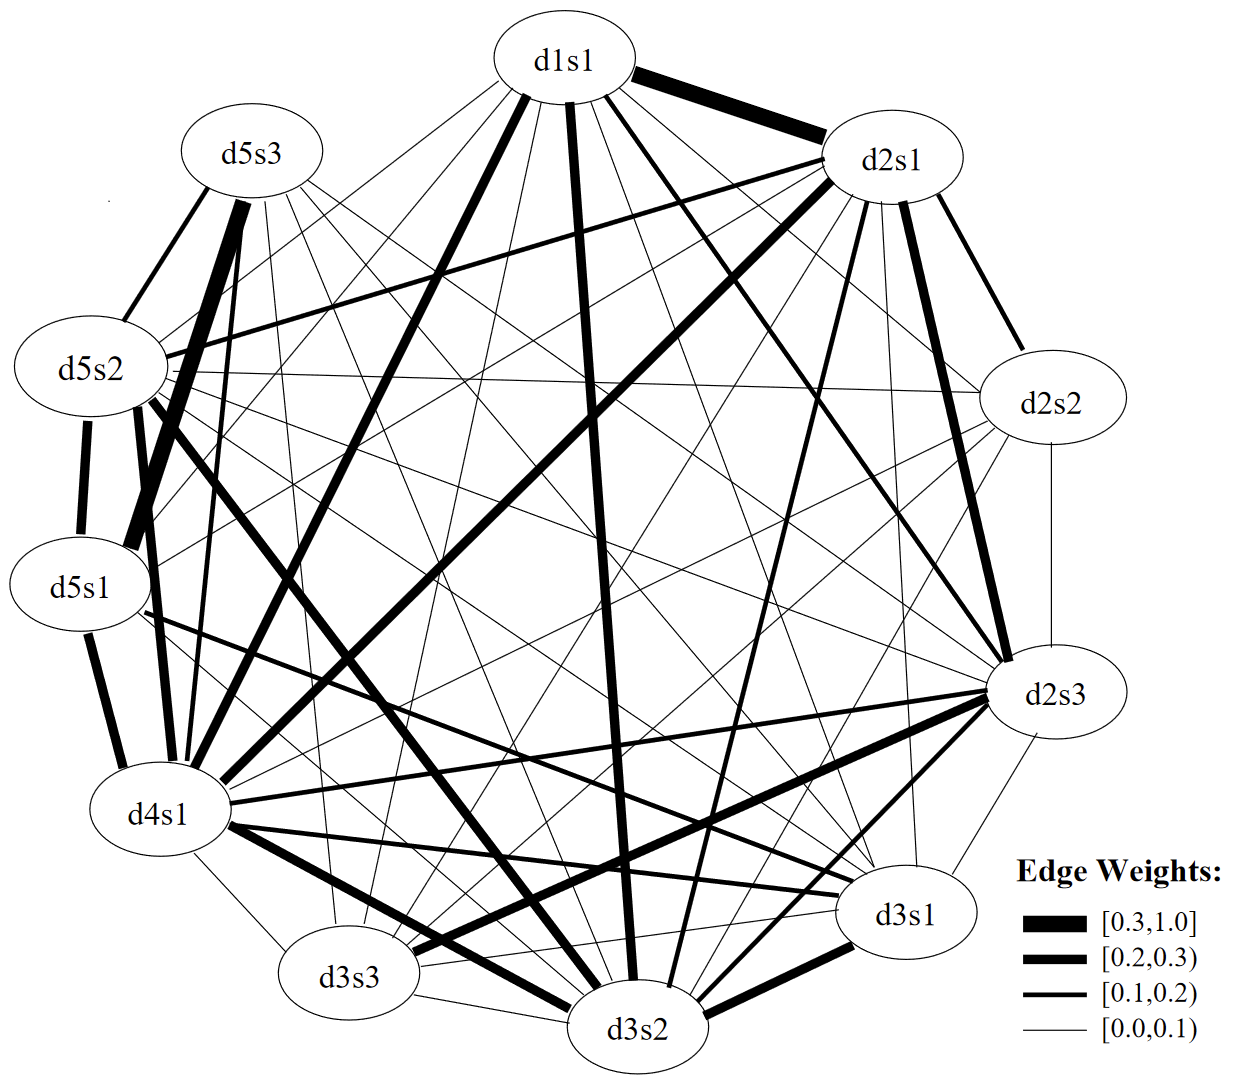
\includegraphics[width=0.5\linewidth]{rys03/lexrank.png}
			\caption{Graf ważony miarą podobieństwa między zdaniami (wierzchołkami)\cite{LexRank}}\label{fig:lexrank}
		\end{figure}
		Graf przedstawiony w postaci macierzy, po znormalizowaniu wierszy, jest macierzą stochastyczną
			(macierz kwadratowa, w której każdy wiersz sumuje się do wartości 1), którą można potraktować jako łańcuch Markova.
		Udowodnione jest, że łańcuch Markova jest zbieżny do rozkładu stacjonarnego, jeśli spełniony jest następujący warunek:
		\[\lim_{x \to \infty}X^n = 1^T r\]
		gdzie \(X\) to macierz stochastyczna, a \(r\) to rozkład stacjonarny łańcucha Markova.
		Rozkład stacjonarny można interpretować jako prawdopodobieństwo że skończymy na danym elemencie przechodząc przez łańcuch, niezależnie od stanu początkowego.
		Możemy go więc potraktować jako wektor centralny (ang.\ \emph{centrality vector}),
			gdzie wartość każdego elementu informuje, jak bardzo centralne jest zdanie na danej pozycji.

		W oryginalnej pracy autorzy mierzyli odległości pomiędzy wektorami TF-IDF\@.
		Nic nie stoi jednak na przeszkodzie, aby w ich miejsce wstawić wektory wygenerowane przez model BERT\@.
		Otrzymany w ten sposób wektor centralny posłuży jako wagi wektorów zdań oraz jako ranking.

	\subsection{TF-IDF}
		Alternatywną metodę ważenia zdań oparto na metodzie TF-IDF\@.
		TF odnosi się do \emph{term-frequency} i oznacza częstość występowania danego słowa w dokumencie.
		IDF oznacza \emph{inverse document-frequency}, zawiera wartości dla każdego słowa, informujące jak bardzo jest ono powszechne.
		Im w większej liczbie dokumentów występuje dane słowo, tym mniej informacji niesie o konkretnym dokumencie.
		Wartość IDF obliczana jest według następującego wzoru:
		\[idf(t)=\log\left(\frac{1+n}{1+df(t)}\right) + 1\]
		gdzie \(t\) oznacza słowo, \(n\) to liczba wszystkich dokumentów, a \(df(t)\) to częstość występowania słowa we wszystkich dokumentach.
		Wartość \(tfidf(t)\) obliczana jest jako iloczyn \(tf(t)\) i \(idf(t)\).
		
		W pierwszym kroku wyuczono model na całym korpusie, aby skonstruować pełen słownik oraz wartości macierzy IDF\@.
		Następnie podczas generowania wektorów wypowiedzi, obliczana jest macierz tf-idf, gdzie wierszami są kolejne zdania.
		Dla każdego zdania kolumny są sumowane, dzięki czemu otrzymujemy wektor o długości równej liczbie zdań oznaczający,
			na ile znaczące są słowa w zdaniu w kontekście całego korpusu (macierz IDF zawiera wartości uwzględniające wszystkie dane).
		Sama ta wartość nie może posłużyć jednak do porównywania zdań, gdyż dłuższe zdania będą miały wyższy wynik, nawet jeśli będą złożone z samych nieznaczących słów.
		Podzielenie tych wartości przez liczę wykrytych słów w danym zdaniu (liczbę niezerowych kolumn w danym wierszu macierzy tf-idf) będzie miało odwrotny efekt
			--- preferowane będą krótkie zdania z małą liczbą słów o wysokim wyniku tf-idf.
		Dłuższe zdania, które mogą zawierać istotne informacje, będą miały niski wynik, gdyż naturalnie składają się również z mniej znaczących słów.
		Postanowiono więc zbadać, jak zmienia się suma wartości tf-idf w zależności od liczby wykrytych słów.
		Zależność ta przedstawiona została na wykresie~\ref{fig:tfidf_sent}a.
		Poprzez aproksymację punktową do danych dopasowana została funkcja potęgowa narysowana na wykresie kolorem czerwonym.
		Aproksymacji poddane zostały trzy współczynniki według następującego wzoru funkcji:
		\[a\cdot x^b + c\]
		dzięki czemu otrzymano następującą funkcję, której dobrym przybliżeniem jest pierwiastek kwadratowy:
		\[1.003\cdot x^{0.486} - 0.065\]
		Odzwierciedla ona średnią sumę wartości tf-idf dla danej długości zdania.
		Można więc przyjąć, że zdania poniżej tej krzywej są mniej istotne, niż zdania powyżej.
		Wartości wszystkich zdań normalizowane są wartością tej funkcji, dzięki czemu nie są promowane ani długie zdania, ani krótkie.
		Znormalizowane wartości zdań przedstawione zostały na wykresie~\ref{fig:tfidf_sent}b.
		Wartości te użyte zostały jako wagi wektorów BERT oraz jako ranking zdań.

		\begin{figure}[htb]
			\centering
			\begin{minipage}{.5\textwidth}
				a)\par\medskip % chktex 10
				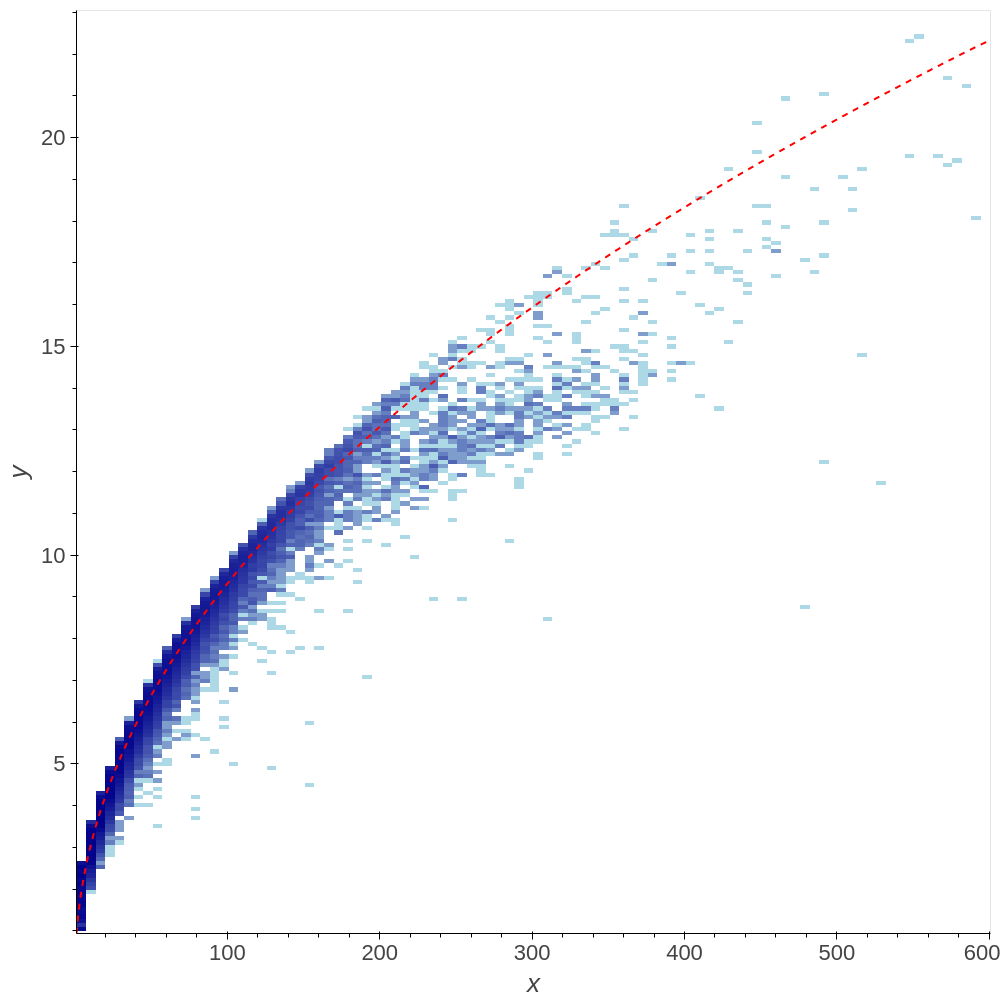
\includegraphics[width=\linewidth]{rys03/tfidf.png}
			\end{minipage}%
			\begin{minipage}{.5\textwidth}
				b)\par\medskip % chktex 10
				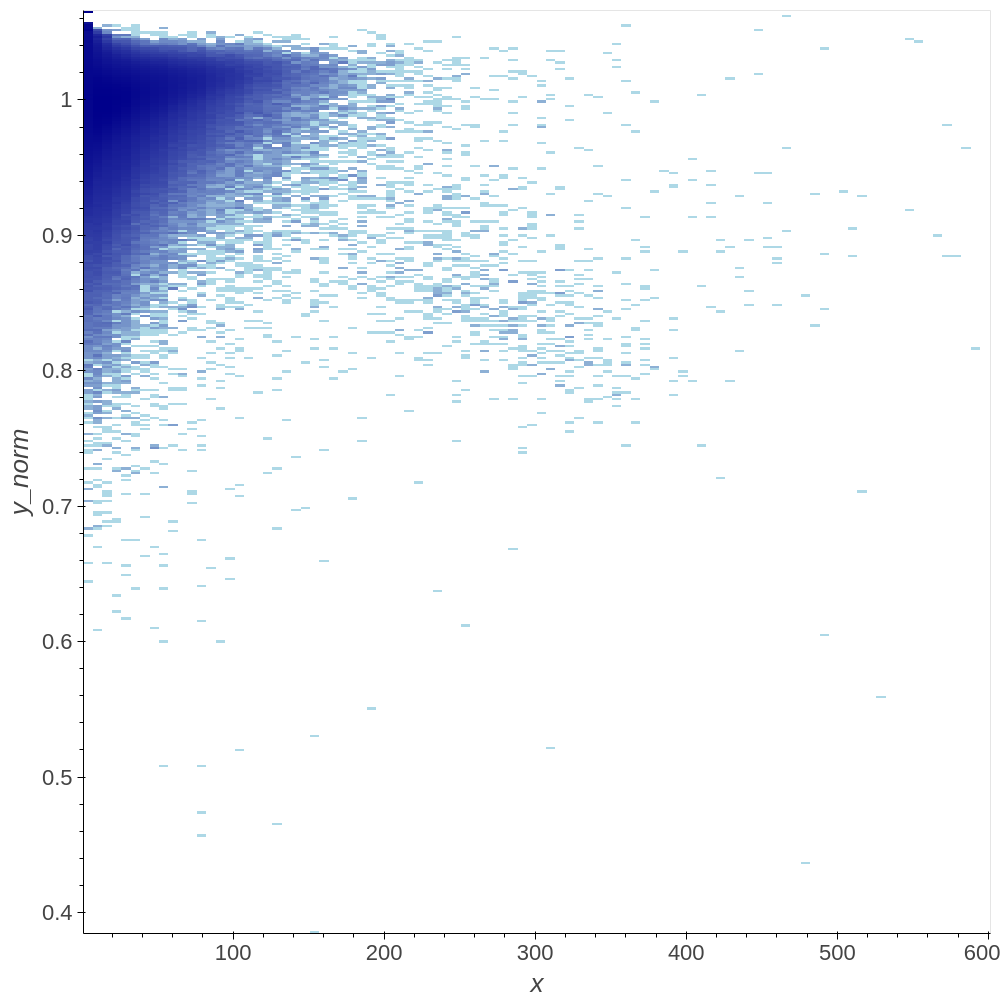
\includegraphics[width=\linewidth]{rys03/tfidf_norm.png}
			\end{minipage}
			\caption{Suma wartości tf-idf w zależności od liczby wykrytych słów (zakres do 600 słów):
				a) dane nieznormalizowane z dopasowaną krzywą, b) dane znormalizowane krzywą}\label{fig:tfidf_sent} % chktex 9 chktex 10
		\end{figure}

\section{Alternatywne rozwiązania}
	Modele oparte o transformery zajmują obecnie wysokie miejsca w rankingach, jednak nie są to jedyne metody dające dobre wyniki.
	W celu porównania wyników wygenerowano wektory dwoma alternatywnymi metodami --- siecią konwolucyjną oraz standardowym TF-IDF\@.

	\subsection{Sieć konwolucyjna}
		Sieci konwolucyjne wykorzystują warstwy połączone filtrami konwolucyjnymi nakładanymi na lokalne cechy.
		Początkowo wykorzystywane do zagadnień związanych z przetwarzaniem obrazów,
			znalazły zastosowanie również w pozostałych dziedzinach uczenia maszynowego, w tym NLP\@.
		W 2019r. Google udostępniło wielojęzykowy wariant modelu USE (ang.\ \emph{Universal Sentence Encoder})\cite{use_multilingual} wspierający 16 języków, w tym polski.
		W pracy tej opisano dwa warianty --- jeden wykorzystujący CNN oraz drugi opierający się na transformerach.
		Model oparty na transformerach osiągnął drugi najlepszy wynik w zadaniu SICK-R w polskim rankingu Polish Sentence Evaluation\cite{sentence_eval}.
		Wersja CNN modelu jest szybsza kosztem mniejszej dokładności.
		Umożliwia ona jednak kodowanie znacznie dłuższych zdań (256 tokenów kontra 100).
		Oba modele wytrenowane zostały na danych zebranych z forów dyskusyjnych (w postaci pytania i odpowiedzi)
			oraz na zbiorze SNLI (Stanford Natural Language Inference) przetłumaczonym na pozostałe 15 języków za pomocą Google Translate.

	\subsection{TF-IDF}
		W przeciwieństwie do omawianych wyżej modeli, w przypadku TF-IDF długość wypowiedzi działa na korzyść algorytmu.
		Im dłuższa wypowiedź, tym większa szansa na uzyskanie kombinacji słów dokładniej identyfikującej dokument.
		Algorytm ten nie posiada żadnego górnego ograniczenia na długość dokumentu.
		Algorytm podczas zliczania liczby wystąpień danego słowa nie bierze pod uwagę odmian słów,
			przez co słowa ,,budżet'' i ,,budżetu'' są traktowane jako osobne kategorie.
		Jest to szczególnie istotne w językach słowiańskich, ponieważ wykorzystywanych jest w nich mnóstwo odmian słów.
		
		Aby zminimalizować wynikającą z tego działania utratę informacji, zdecydowano się wstępnie przetworzyć dokumenty przed zliczeniem słów.
		Wykorzystano w tym celu polski model do biblioteki \verb|spaCy|
			--- \verb|pl_spacy_model_morfeusz|\cite{spacy_pl} udostępniony przez Instytut Podstaw Informatyki Polskiej Akademii Nauk\footnote{\url{http://zil.ipipan.waw.pl/SpacyPL} (dostęp dnia 21 maja 2021)}.
		Biblioteka umożliwia między innymi lematyzację (sprowadzenie słowa do formy podstawowej) każdego słowa w zdaniu.
		Wykorzystuje przy tym wyuczony model, który rozpoznaje strukturę zdania --- przykładowo, czy dane słowo jest w danym kontekście rzeczownikiem, czy czasownikiem.
		Następnie na podstawie tej wiedzy może określić formę podstawową słowa.
		Polski model na tym etapie wykorzystuje słownik morfologiczny Morfeusz2\cite{morfeusz}.
		Zbudowany jest on na danych ze Słownika gramatycznego języka polskiego.

		Podczas tokenizacji dokumentów generowane są również n-gramy z zakresu (1,3).
		Oznacza to, że zliczane będą również wystąpienia dwóch oraz trzech kolejnych słów (np. ,,Unia Europejska'', ,,Rzecznik praw obywatelskich'').
		Dodatkowo, przyjęto próg odrzucenia \verb|min_df| równy 5 oznaczający, że dany token musi wystąpić w minimum pięciu dokumentach,
			aby był uwzględniony w wynikowej macierzy.
